\documentclass[UTF8]{ctexart}

\usepackage{subfigure}
\usepackage{listings}
\usepackage{color}
\usepackage{shapepar}
\usepackage{bbm}
\usepackage{graphicx}
\usepackage{amsmath}
\usepackage{CJKfntef}

\definecolor{dkgreen}{rgb}{0,0.6,0}
\definecolor{gray}{rgb}{0.5,0.5,0.5}
\definecolor{mauve}{rgb}{0.58,0,0.82}

\lstset{ %
  language=Octave,                % the language of the code
  basicstyle=\footnotesize,           % the size of the fonts that are used for the code
  numbers=left,                   % where to put the line-numbers
  numberstyle=\tiny\color{gray},  % the style that is used for the line-numbers
  stepnumber=2,                   % the step between two line-numbers. If it's 1, each line 
                                  % will be numbered
  numbersep=5pt,                  % how far the line-numbers are from the code
  backgroundcolor=\color{white},      % choose the background color. You must add \usepackage{color}
  showspaces=false,               % show spaces adding particular underscores
  showstringspaces=false,         % underline spaces within strings
  showtabs=false,                 % show tabs within strings adding particular underscores
  frame=single,                   % adds a frame around the code
  rulecolor=\color{black},        % if not set, the frame-color may be changed on line-breaks within not-black text (e.g. commens (green here))
  tabsize=2,                      % sets default tabsize to 2 spaces
  captionpos=b,                   % sets the caption-position to bottom
  breaklines=true,                % sets automatic line breaking
  breakatwhitespace=false,        % sets if automatic breaks should only happen at whitespace
  title=\lstname,                   % show the filename of files included with \lstinputlisting;
                                  % also try caption instead of title
  keywordstyle=\color{blue},          % keyword style
  commentstyle=\color{dkgreen},       % comment style
  stringstyle=\color{mauve},         % string literal style
  escapeinside={\%*}{*)},            % if you want to add LaTeX within your code
  morekeywords={*,...}               % if you want to add more keywords to the set
}










\usepackage{underscore}
\usepackage{fancyhdr}
\usepackage{extramarks}
\usepackage{amsmath}
\usepackage{amsthm}
\usepackage{amsfonts}
\usepackage{tikz}
\usepackage[plain]{algorithm}
\usepackage{algpseudocode} 
\usepackage{graphicx}
\usepackage{dsfont}
\usepackage{listings}
\lstset{language=Matlab}%代码语言使用的是matlab
\lstset{breaklines}%自动将长的代码行换行排版
\lstset{extendedchars=false}%解决代码跨页时,章节标题,页眉等汉字不显示的问题
\usetikzlibrary{automata,positioning}

\topmargin=-0.45in
\evensidemargin=0in
\oddsidemargin=0in
\textwidth=6.5in
\textheight=9.0in
\headsep=0.25in

\linespread{1.1}

\pagestyle{fancy}
\lhead{\hmwkAuthorName}
\rhead{\hmwkClass \:\hmwkTitle}
\cfoot{\thepage}

\renewcommand\headrulewidth{0.4pt}
\renewcommand\footrulewidth{0.4pt}

\setlength\parindent{0pt}


\newcommand{\enterProblemHeader}[1]{
    \nobreak\extramarks{}{问题\arabic{#1} continued on next page\ldots}\nobreak{}
    \nobreak\extramarks{问题 \arabic{#1} (continued)}{Problem \arabic{#1} continued on next page\ldots}\nobreak{}
}

\newcommand{\exitProblemHeader}[1]{
    \nobreak\extramarks{问题 \arabic{#1} (continued)}{Problem \arabic{#1} continued on next page\ldots}\nobreak{}
    \stepcounter{#1}
    \nobreak\extramarks{问题 \arabic{#1}}{}\nobreak{}
}

\setcounter{secnumdepth}{0}
\newcounter{partCounter}
\newcounter{homeworkProblemCounter}
\setcounter{homeworkProblemCounter}{1}
\nobreak\extramarks{ \arabic{homeworkProblemCounter}}{}\nobreak{}

\newenvironment{homeworkProblem}{
   %\section{ \arabic{homeworkProblemCounter}}
   %\setcounter{partCounter}{1}
    \enterProblemHeader{homeworkProblemCounter}
}{
    \exitProblemHeader{homeworkProblemCounter}
}


\newcommand{\hmwkTitle}{DELS}
\newcommand{\hmwkClass}{MATLAB}
\newcommand{\hmwkClassTime}{}
\newcommand{\hmwkAuthorName}{郭龙昕,江诗毅,胡进}
\title{
    \vspace{2in}
    \textmd{\textbf{\hmwkClass:\ \hmwkTitle}}\\
    \vspace{0.1in}\large{\textit{ \hmwkClassTime}}
    \vspace{3in}
}
\author{\textbf{\hmwkAuthorName}}

\begin{document}

\maketitle

\pagebreak

\begin{homeworkProblem}

\section{任务一}
\subsection{解决思路}

\begin{itemize}
\item[1] 计算$m$期生产满足到第$n-1$期的成本。
\item[2] 计算从第$1$期开始到第$N$最低成本。
\item[3] 输出从第$1$期开始到第$N$的最优生产路径。
\item[4] 检查一个路线是否是最优路线
\end{itemize}

\subsection{具体实现过程}
\begin{itemize}
\item 计算$m$期生产满足到第$n-1$期的成本。
\normalem{程序:mToNCost.m}
\begin{lstlisting}
function cost = mToNCost(d,k,c,h,m,n)
%
%输入:
%   d(vector) : 各阶段的需求
%   k(vector) : 各阶段的固定成本
%   c(vector) : 各阶段的单位边际成本
%   h(vector) : 各阶段的持有库存的边际成本
%   m(number) : 开始的阶段
%   n(number) : 结束的后一阶段
%
%输出:
%   cost(number) : 第m期生产满足第m到n-1期的所有需求带来的成本
for i = m:n-1
  cost = cost + c(m) .* d(i) + sum(h(m:i-1)) .* d(i);
end
end
\end{lstlisting}

\item 计算从第$1$期开始到第$N$最低成本。

\emph{程序:dySolution.m}

\begin{lstlisting}
%算法时间复杂度为O(n^2),n为维度
%输入:
%   d(vector) : 各阶段的需求
%   k(vector) : 各阶段的固定成本
%   c(vector) : 各阶段的单位边际成本
%   h(vector) : 各阶段的持有库存的边际成本
%
%输出:
%   result(number) : 最小成本
%   road(vector) : 达到最小成本的方案(0代表不生产,1代表生产)
%
%example(d,k,c,h都为n维向量):
%   [optResult,road] = dySolution(d,k,c,h)
function [result,road] = dySolution(d,k,c,h)
    disp('璇疯緭鍏ョ淮搴︾浉鍚岀殑鍚戦噺');
    result = -1;
    road = -1;
    return 
end
s = zeros(1,length(d));
for i = 1:length(d)
    r(i) = mToNCost(d,k,c,h,1,i+1);
    s(i) = 1;
    for j = 1:i-1
        temp = r(j) + mToNCost(d,k,c,h,j+1,i+1);
        if temp < r(i) 
            r(i) = temp;
            s(i) = j+1;
        end
    end
end
result = r(length(d));
road = dyRoad(length(d),s);
end
\end{lstlisting}

\emph{步骤}
\begin{itemize}
    \item[1] 基本的输入向量验证,例如 验证维度是否符合要求。
    \item[2] 预分配内存,提高效率:一维数组r表示从第1期到第n期的最小成本,该问题是动态规划的子问题。一维数组s表示r(n)对应最优子方案中最后一次生产的时期是在第s(n)阶段。
    \item[3] 迭代求解子问题,例如现在是第i次循环,依次遍历s(i)= 1 to i,计算值,记录下最优路线方案,以及最有成本。
    \item[4] 重复步骤3,直到r(n)被算出,停止迭代。
\end{itemize}

\item{输出从第$1$期开始到第$N$的最优生产路径}
\emph{程序:dyRoad.m}
\begin{lstlisting}
function road = dyRoad(leng,s)
%dyRoad - 鏍规嵁鍔ㄦ�瑙勫垝缁欏嚭鐨剆锛岄�褰掔殑缁欏嚭鏈�紭鍐崇瓥鏂规
%
%璺緞鐨勯�褰掑畾涔夛細 1 ---> ... ---> s(s(n) - 1) --->  s(n) ---> N 
%杈撳叆锛�%   leng(number):闃舵鏁扮洰
%   s(vector):鍦ㄥ姩鎬佽鍒掔畻娉曚腑缁欏嚭鐨剆
%杈撳嚭锛�%   road(vector) : 杈惧埌鏈�皬鎴愭湰鐨勬柟妗�0浠h〃涓嶇敓浜э紝1浠h〃鐢熶骇)

road = zeros(1,leng);
point = leng;
while point > 0 
    road(s(point)) = 1;
    point = s(point) - 1;
end
end
\end{lstlisting}
\emph{步骤}
\begin{itemize}
    \item[1] 路径的递归定义: 1 ---> ... ---> s(s(n) - 1) --->  s(n) ---> N 
    \item[2] 从s(n)开始,表示最后生产的阶段。
    \item[3] 继续计算s( s(n)-1 ),表示倒数第二次的生产阶段。
    \item[4] 重复下去,直到回到s(i) - 1 < 0。 
\end{itemize}

\item 检查一个路线是否是最优路线

首先对为什么要编写程序检查一个路线是否是最优路线作出解释:
由于对于每组d,k,c,h都有可能有多个最优解,所以我们有时候需要核查给定road是否是最优方案的方法。


\emph{程序:checkOptRoad.m}
\begin{lstlisting}
%checkOptRoad - 判断给定路径是否是动态规划的最优解
%
%输入:
%   d(vector) : 各阶段的需求
%   k(vector) : 各阶段的固定成本
%   c(vector) : 各阶段的单位边际成本
%   h(vector) : 各阶段的持有库存的边际成本
%   road(vector) : 路线
%
%输出:
%   result(boolean) : 逻辑1或者逻辑0
% 根据路线给出成本
% 比较最优成本与sum_cost
function result = checkOptRoad(d,k,c,h,road)
plan = find(road == 1);
sum = 0;
for i = 1:length(plan)-1
    sum = sum + mToNCost(d,k,c,h,plan(i),plan(i+1));
end
sum = sum + mToNCost(d,k,c,h,plan(length(plan)),length(d)+1);
% disp(sum);
% disp(dySolution(d,k,c,h));
result = sum == dySolution(d,k,c,h);
end
\end{lstlisting}

\end{itemize}

\subsection{测试主程序}


\emph{测试程序伪代码}

\begin{lstlisting}
% 随机生成d,k,c,h,以及c,h增加的同一个常数add
% 生成1000组测试用例
d,k,c,h,add = randi(10,1000,10);

for i = 1:1000
% 分别计算四种情况下的最优值
	[a1,b1] = dySolution(d(i,:),k(i,:),c(i,:),h(i,:));
	[a2,b2] = dySolution(d(i,:),k(i,:) + tem,c(i,:),h(i,:));
	[a3,b3] = dySolution(d(i,:),k(i,:),c(i,:) + tem,h(i,:));
	[a4,b4] = dySolution(d(i,:),k(i,:)+tem,c(i,:)+tem,h(i,:));
% 检验他们的最优决策方案是否相同
all([
	checkOptRoad(d(i,:),k(i,:),c(i,:) + tem,h(i,:),b1),
	checkOptRoad(d(i,:),k(i,:) + tem,c(i,:),h(i,:),b1),
	checkOptRoad(d(i,:),k(i,:) + tem,c(i,:)+tem,h(i,:),b1)
]) == 1
\end{lstlisting}

\emph{测试结果}

\begin{tabular}{c c c}
	\hline
	测试用例 & 结果 & 要求 \\
	dySolution(1,1,1,1) & 通过 & 结果为2 \\
	dySolution(d,k,c,h) & 通过 & d,k保持不变,c或者h增加一个常数,最优方案不变 \\
	dySolution(d,k,c,h) & 通过 & k=0,c,h保持不变,d不影响最优决策 \\
	\hline
\end{tabular}

\subsection{算法效率分析}

对于该算法,在每次子问题的迭代过程中,都要计算i-1种方案进行对比,所以算法的复杂度是$O(n^2)$。下面我们绘制出该算法解决问题所需时间随规模变化的曲线。(图1,图2)


稀疏点拟合的参数分别为\(a=0.0000\cdot 10^{-4}\quad b=-0.0058\cdot 10^{-4}\quad c=0.1412\cdot 10^{-4}\),如图一:稀疏点拟合。

密集点拟合的参数分别为\(a=0.0000\cdot 10^{-4}\quad b=-0.0065\cdot 10^{-4}\quad c=0.1921\cdot 10^{-4}\),如图二:密集点拟合。


\begin{figure}[H] 
	\centering
	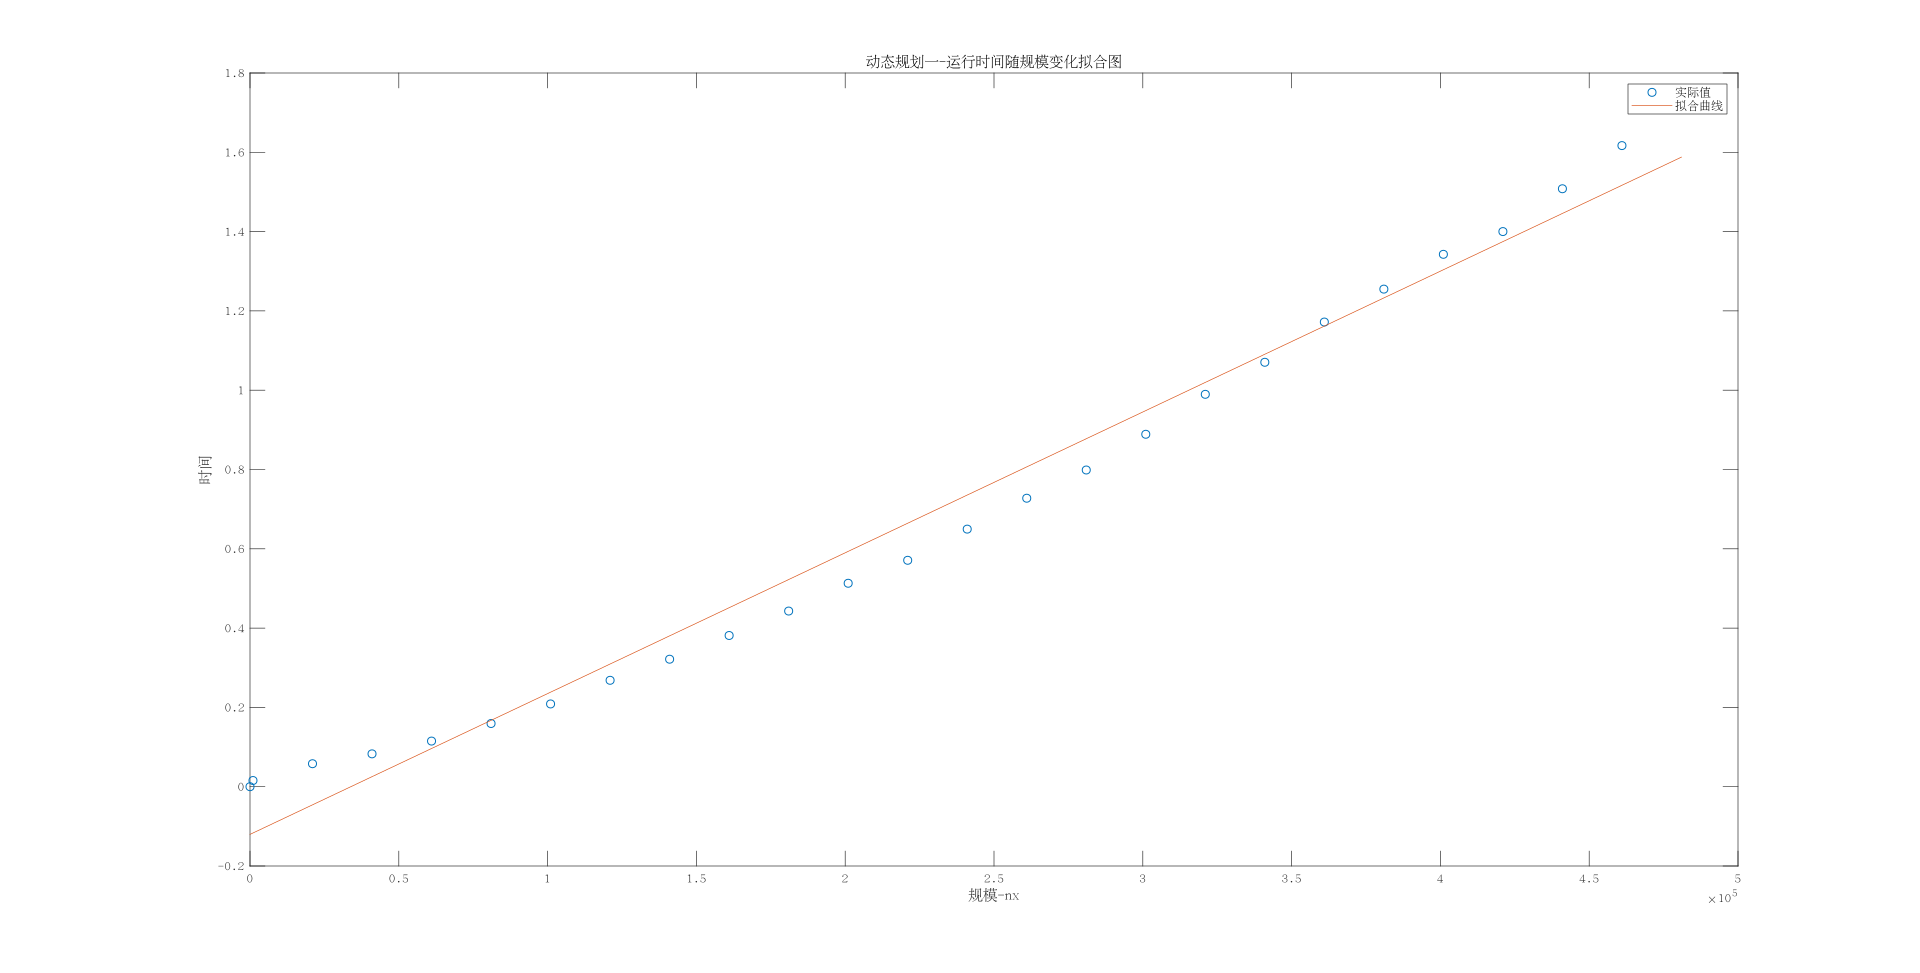
\includegraphics[width=12cm]{1.jpg}
	\caption{稀疏点拟合}
\end{figure}


\begin{figure}
		\centering
		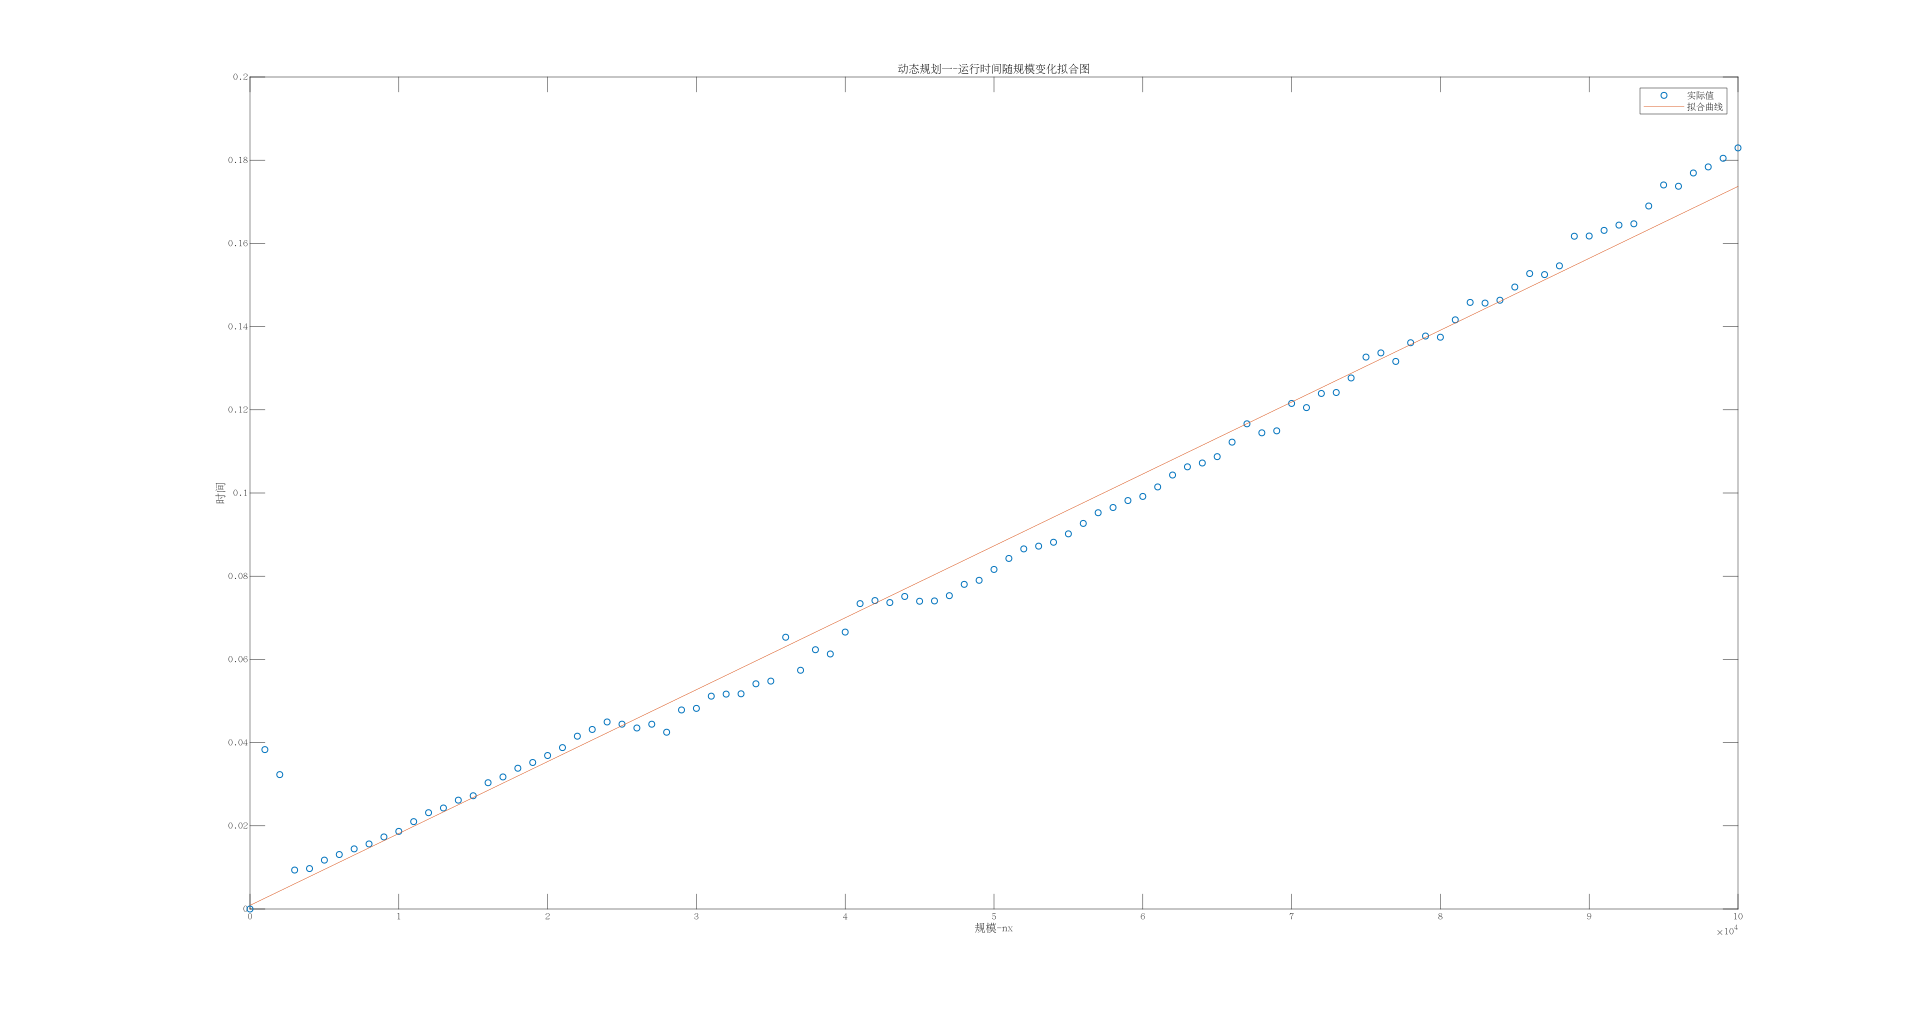
\includegraphics[width=12cm]{2.jpg}
		\caption{密集点拟合}
\end{figure}

\section{任务二}

\begin{itemize}
\item[\textbf{a}] \textbf{如果没有固定生产成本,那么最优生产序列与需求序列无关。}
\begin{itemize}
\item[1] \normalem{数值分析:}

测试命题是否正确的伪代码
\begin{lstlisting}
% 测试 k = 0时,最优决策与d无关。
d = randi(10,100,10);
k = zeros(1,10);
c = randi(10,1,10);
h = randi(10,1,10);
 
[opt,plan] = dySolution(d(1,:),k,c,h);
for i = 1:100
% 检验最优决策方案是否发生改变。
checkOptRoad(d(i,:),k,c,h,plan)
\end{lstlisting}

\item[2] \normalem{数学分析}

假设在$m$期购买第$t$期所需的商品,总费用为:

$$c(m)=k_m+c_md_t+(h_m+h_{m+1}+\cdots + h_{t-1})d_t$$

所要做的决策是选择在某一期订购使得每件商品的平均成本最小。设所做出的最优决策为在第$p$期订购,则

$$p = \mathop{\arg\min}_m \{\frac{c(m)}{d_t}\}=\mathop{\arg\min}_m \{\frac{k_m}{d_t}+c_m+h_m+h_{m+1}+\cdots+h_{t-1}\}$$
 
当$k_m=0$时,最优决策为:
$$p = \mathop{\arg\min}_m \{c_m+h_m+h_{m+1}+\cdots+h_{t-1}\}$$
最优决策的表达式中不含$d_m$,所以当$k_m=0$时,第$m$期的最优决策与$d_m$无关。

所以当$k_n=0,\forall n $时,最优生产计划与需求序列无关。

\end{itemize}

\item[\textbf{b}] \textbf{在计算第m期生产从第m期至第n期所需的所有商品的总成本的时,有两种思路,一种是分别计算从第m期至第n-1期间各期成本,然后再求和;另一种是除固定成本外,先分别计算满足各批次需求的成本,然后再求和。一般而言,用第m期的生产来满足第$t \ge m$期需求的总成本可记录为$c_{m.t}d_t$。请给出一般形式的$c_{m,t}$表达式,然后再Matlab中实现,并用原来的代码测试。}

$c_{m,t}$的表达式如下:
$$c_{m,t}=c_m+h_m+h_{m+1}+\cdots+h_{t-1}$$
使用这种思路写出的totalcost函数为:

\begin{lstlisting}
function m_n_totalcost = totalcost_2(d,k,c,h,m,n)
%求出在第m期生产m-(n-1)期的所有产品的总花费
%输入:
%  d(vector) : 需求序列
%  k(vector) : 每一期生产的固定成本
%  c(vector) : 每一期生产单位商品的成本
%  h(vector) : 每一期期末单位商品的库存成本
%  m(number) : 开始的期数
%  n(number) : 结束期数的下一期。
%
%输出:
%  m_n_totalcost(number) : 第m期生产满足第m到n-1期的所有需求的总成本
m_n_totalcost = k(m) ; 
for i = m:n-1
   m_n_totalcost =m_n_totalcost + c(m) .* d(i) + sum(h(m:i-1)) .* d(i);
end
end
\end{lstlisting}
下面对上述代码进行测试

测试思路:对于相同的d,k,c,h分别调用第一种思路下的totalcost函数,和第二种思路下的totalcost_2函数,比较得出的函数值是否相同,如果不同,那么函数会报错,并跳出循环,如果没有报错,重复10000次。

测试代码如下:
\begin{lstlisting}
for i = 1 : 10000
d = randi([1,100],1,10) ;
c = randi([1,100],1,10) ;
k = randi([1,100],1,10) ;
h = randi([1,100],1,10) ;
a = totalcost(d,k,c,h,1,9);
b = totalcost_2(d,k,c,h,1,9);
if a ~= b
    disp('程序有误')
    break
end
end
\end{lstlisting}
运行结果:程序没有报错,说明上述程序totalcost_2是正确的。

\item[\textbf{c}] \textbf{如果把$\ell(m.n)$的定义改成$\ell(m,n)=k_m+c_{m,N+1}d_{1,n+1}$,是否会改变原问题的最优解。}

在解决这个问题的时候,我们将老师给的式子代入程序运算后发现最优解会发生改变。

但是我们进一步猜测应该具有某个,甚至某一类表达式是的最优解不发生改变,我们尝试对老师给出的表达式进行变形,主要改变$c,d$的下标。我们试过的表达式有$\ell(m,n)=k_m+c_{m,N+1}d_{1,n+1},\ell(m,n)=2k_m+c_{m,N+1}d_{1,n+1},\ell(m,n)=k_m+c_{m,N+1}d_{m,n+1},\ell(m,n)=k_m+c_{m,N+1}d_{m,n},\ell(m,n)=k_m+c_{m,N+1}d_{m,n-1}$,最后发现当表达式变为$\ell(m,n)=k_m+c_{m,N+1}d_{m,n-1}=k_m+(c_m+h_m+h_{m+1}+\cdots+h_N)(d_m+d_{m+1}+\cdots+d_{n-1})$最优解不发生改变。

\textbf{下面我们证明:当表达式为$\ell(m,n)=k_m+c_{m,N+1}d_{m,n-1}=k_m+(c_m+h_m+h_{m+1}+\cdots+h_N)(d_m+d_{m+1}+\cdots+d_{n-1})$最优解不发生改变。}
\begin{itemize}
\item[1] \normalem{数值分析}

我们将上述函数totalcost改为题目中的$\ell(m,n)=k_m+c_{m,N+1}d_{m,n-1}$,得到一个新的函数,我们将其命名为totalcost_3。

程序如下
\begin{lstlisting}
function m_n_totalcost = totalcost_3(d,k,c,h,m,n)
%求出在第m期生产m-(n-1)期的所有产品的总花费
%输入:
%   d(vector) : 需求序列
%   k(vector) : 每一期生产的固定成本
%   c(vector) : 每一期生产单位商品的成本
%   h(vector) : 每一期期末单位商品的库存成本
%   m(number) : 开始的期数
%   n(number) : 结束期数的下一期。
%
%输出:
%   m_n_totalcost(number) : 第m期生产满足第m到n-1期的所有需求的总成本
m_n_totalcost = k(m) + (c(m)+sum(h(m:length(h))))  .* sum(d(m:n-2)) ;
end
\end{lstlisting}

当总成本为totalcost_3给出的成本时,我们测试最优解是否不变。

程序思路:

在总成本分别为totalcost_3和totalcost给出的成本时,我们分别调用DELS函数,如果最优解不同,那么程序报错并跳出循环;如果最优解相同,那么重复10000次。

程序:totalcost_3_text
\begin{lstlisting}
for i = 1 :10000
    d = randi([1,100],1,10) ;
    k = randi([1,100],1,10) ;
    c = randi([1,100],1,10) ;
    h = randi([1,100],1,10) ;
    [a,b] = DELS(d,k,c,h) ;
    [c,d] = totalcost_3_DELS(d,k,c,h) ;
    if b~=d
        disp("命题错误")
        break
    end
end
\end{lstlisting}

运行结果:程序没有报错。

这就证明了在$\ell(m,n)$换成新的表达式以后,最优解没有发生改变。

\item[2] \normalem{数学分析}

在原来的$\ell(m,n)$的定义下,

假设在$m$期购买第$n$期所需的商品,总费用为:

$$c(m,n)=k_m+c_md_n+(h_m+h_{m+1}+\cdots + h_{n-1})d_n$$

所要做的决策是选择在某一期订购使得总成本最小。设所做出的最优决策为在第$p$期订购,则

$$p(n) = \mathop{\arg\min}_m \{ c(m,n)\}=\mathop{\arg\min}_m \{k_m+(c_m+h_m+h_{m+1}+\cdots+h_{n-1})d_n\}$$

在新的$\ell(m,n)$的定义下,在第$m$期生产第$m$期到第$n$期所需所有产品的总费用为:
$$\ell(m,n+1)=k_m+(c_m+h_m+\cdots+h_N)(d_m+d_{m+1}+\cdots+d_n)$$
其中$N$为问题所求的总得期数。

此时,在第$m$期生产第$n$期所需的产品的总费用为:
$$c(m,n)=k_m+(c_m+h_m+\cdots+h_N)d_n$$
所做出的决策为选择第$m$期生产第$n$期所需的产品,使得总成本最小,即
$$\begin{aligned}p(n)&= \mathop{\arg\min}_mc(m,n) \\ &=\mathop{\arg\min}_m\{ k_m+(c_m+h_m+\cdots+h_N)d_n \}\\
&=\mathop{\arg\min}_m\{k_t+(c_m+h_m+h_{m+1}+\cdots+h_{n-1})d_n+(h_n+h_{n+1}+\cdots+h_N)d_n\}
\  \  \  \text{(1)} \\ &=\mathop{\arg\min}_m\{k_t+(c_m+h_m+h_{m+1}+\cdots+h_{n-1})d_n\}
\end{aligned}$$
(1)式中有两项构成,一项为$k_t+(c_m+h_m+h_{m+1}+\cdots+h_{n-1})d_n$这正是在原来的$\ell(m,n)$定义下在$m$期订购第$n$期所需商品的总费用,而另一项为$(h_n+h_{n+1}+\cdots+h_N)d_n$这是一个与$m$无关的常数。

所以在以前的$\ell(m,n)$的定义下,如果在$p(n)$期订购第$n$期所需商品使得总成本最小,那么在新的$\ell(m,n)$的定义下,同样在$p(n)$期订购第$n$期所需商品使得总成本最小。

由于$n$的任意性,该结论对$1-N$期都成立。

即,在改变$\ell(m,n)$的定义下,最优解不会改变。
\end{itemize}

\subsection{任务三}

根据题目提示,如果已经得到了第n期之后的最优生产期分别为 \( n=s_o < s_1 < s_2 < \cdots < s_m \leq N \),那么在计算第n-1期之后的最优生产计划时,\( s_0,s_1 \)可能会更新,但是\( s_2 \)及以后的计划期不会改变。

我们做出猜想:如果已经得到了第m期之前的最优生产期分别为 \( n=s_o < s_1 < s_2 < \cdots < s_n \leq m \),那么在计算第m+1期之后的最优生产计划时,\( s_m,s_{m-1} \)可能会更新,但是\( s_{n-2} \)及之前的计划期不会改变。也就是说最多会改变最近两期的决策。

算例验证如下图所示.

\begin{figure}[H]                 
    \centering
    \begin{minipage}[t]{1\textwidth}
        \centering
        \includegraphics[width=12cm]{11.png}
        \caption{稀疏点拟合}
    \end{minipage}
    \begin{minipage}[t]{1\textwidth}
        \centering
        \includegraphics[width=12cm]{选区_197.png}
        \caption{密集点拟合}
    \end{minipage}
\end{figure}

从图中可以看出最多只有最近两期的决策会发生改变。

据此,我们可以对上面已经提到的算法进行改进:


\subsection{实现思路}

\begin{itemize}
    \item[1] 先计算出第一期,以及第一期到第二期的最优决策值。
    \item[2] 从第三期开始迭代,每次只用分四种情况计算最优值。1. 最近的两期都不生产。2. 最近的二期生产,最近的一期不生产。3. 最近的一期不生产,最近的二期生产。 4. 最近的两期都生产。
    \item[3] 比较上面四个结果,得出最优值以及方案。
\end{itemize}

\subsection{具体实现过程}
\emph{程序:OnDySolution.m}
\begin{lstlisting}
function [result,road] = OnDySolution(d,k,c,h)
    disp('璇疯緭鍏ョ淮搴︾浉鍚岀殑鍚戦噺');
    result = -1;
    road = -1;
    return 
end
s = zeros(1,length(d));
r(1) = mToNCost(d,k,c,h,1,2);
s(1) = 1;
if length(d) <= 2  
    result = r(1);
    road = 1;
    return 
end 
can = mToNCost(d,k,c,h,1,3);
bucan = mToNCost(d,k,c,h,1,2) + mToNCost(d,k,c,h,2,3);
if can <= bucan
    r(2) = can;
    s(2) = 1;
else
    r(2) = bucan;
    s(2) = 2;
for i = 3:length(d)
    z_z = mToNCost(d,k,c,h,s(i-2),i+1) + r(i-2) - mToNCost(d,k,c,h,s(i-2),i-1); 
    z_o = mToNCost(d,k,c,h,s(i-2),i-1) + mToNCost(d,k,c,h,i-1,i+1) + r(i-2) - mToNCost(d,k,c,h,s(i-2),i-1);
    o_z = mToNCost(d,k,c,h,s(i-2),i) + mToNCost(d,k,c,h,i,i+1) + r(i-2) - mToNCost(d,k,c,h,s(i-2),i-1);
    o_o = mToNCost(d,k,c,h,s(i-2),i-1) + mToNCost(d,k,c,h,i-1,i) + mToNCost(d,k,c,h,i,i+1) + r(i-2) - mToNCost(d,k,c,h,s(i-2),i-1);   
    r(i) = min([z_z,z_o,o_z,o_o]);
    switch r(i)
        case z_z
            s(i) = s(i-2);
        case z_o
            s(i) = i;
        case o_z
            s(i) = i-1;
        case o_o
            s(i) = i;
    end
    if mToNCost(d,k,c,h,s(i-1),i+1) + r(i-1) - mToNCost(d,k,c,h,s(i-1),i) <= r(i-1) + mToNCost(d,k,c,h,i,i+1)
        s(i) = s(i-1);
        r(i) = mToNCost(d,k,c,h,s(i-1),i+1) + r(i-1) - mToNCost(d,k,c,h,s(i-1),i);
    else 
        s(i) = i;
        r(i) = r(i-1) + mToNCost(d,k,c,h,i,i+1);
    end
end
result = r(length(d));
road = dyRoad(length(d),s);
end
\end{lstlisting}
\subsection{正确性测试}
\emph{测试程序伪代码:}
\begin{lstlisting}
% 随机生成d,k,c,h,以及c,h增加的同一个常数add
% 生成1000组测试用例
d,k,c,h,add = randi(10,1000,10);

for i = 1:1000
% 分别计算四种情况下的最优值
	[a1,b1] = dySolution(d(i,:),k(i,:),c(i,:),h(i,:));
	[a2,b2] = dySolution(d(i,:),k(i,:) + tem,c(i,:),h(i,:));
	[a3,b3] = dySolution(d(i,:),k(i,:),c(i,:) + tem,h(i,:));
	[a4,b4] = dySolution(d(i,:),k(i,:)+tem,c(i,:)+tem,h(i,:));
% 检验他们的最优决策方案是否相同
all([
	checkOptRoad(d(i,:),k(i,:),c(i,:) + tem,h(i,:),b1),
	checkOptRoad(d(i,:),k(i,:) + tem,c(i,:),h(i,:),b1),
	checkOptRoad(d(i,:),k(i,:) + tem,c(i,:)+tem,h(i,:),b1)
]) == 1
\end{lstlisting}

\textit{测试结果}

\begin{tabular}{c c c}
	\hline
	测试用例 & 结果 & 要求 \\
	OnDySolution(1,1,1,1) & 通过 & 结果为2\\
	OnDySolution(d,k,c,h) & 通过 & d,k保持不变,c或者h增加一个常数,最优方案不变\\	
	OnDySolution(d,k,c,h) & 通过 & k=0,c,h保持不变,d不影响最优决策\\
	\hline
\end{tabular}

\subsection{算法效率分析}
使用该算法时,在计算更大一级的问题时,比其小两级的子问题的最优路线不会发生改变,这样就不用重复计算比较选择那个子问题。相当于所有阶段只计算了一次,算法的复杂度变为O(n).
下面我们对其进行验证:

我们绘制出解决问题所需的时间随规模变化的曲线。(图3,图4)

稀疏点拟合的参数分别为\(k=0.1223 \cdot 10^{-4}\)
密集点拟合的参数分别为\(k=0.6295 \cdot 10^{-4}\)
\begin{figure}[H]                 
		\centering
		\includegraphics[width=14cm]{3.jpg}
		\caption{稀疏点拟合}
\end{figure}

\begin{figure}[H]  
		\centering
		\includegraphics[width=14cm]{4.jpg}
		\caption{密集点拟合}
\end{figure}

\subsection{误差分析}
使用上图中任一结果,分析其均方误差。\( MSE = 0.00023 \)

数据来源如下图5(每一项的误差值)。可知拟合的结果较好,所以不拒绝两个算法复杂度分别为\( O(n^2),O(n) \).



\end{document}
